\section{Theorie}
\label{sec:Theorie}
In der Wellenoptik kommt es zur Beugung von Wellen, wenn diese auf eine Öffnung oder
ein Hindernis in der Größenordnung ihrer Wellenlänge treffen. Beugung bedeutet hierbei,
dass die Wellen von ihrer geraden Ausbreitungsrichtung abgebracht werden und sich in
die bei geradliniger Ausbreitung versperrten Bereiche fortpflanzen. In diesem Versuch
wird das Phänomen der Beugung bei sichtbarem Licht untersucht. \\
Im Folgenden wird stets die Fraunhofer-Näherung angenommen. Das bedeutet, dass das Licht
von einer als punktförmig angenommenen Quelle, die sich weit hinter der Blende befindet,
ausgeht und dass der Abstand des Schirms von der Blende als groß angenommen wird. Dies
entspricht also einer Fernfeldnäherung. Schematisch ist dies in \ref{fig:fraunhofer}
dargestellt. Weil die Quelle als weit entfernt angenommen wird, können eintreffende
Strahlen näherungsweise als parallel angenommen werden.

\begin{figure}
  \centering
  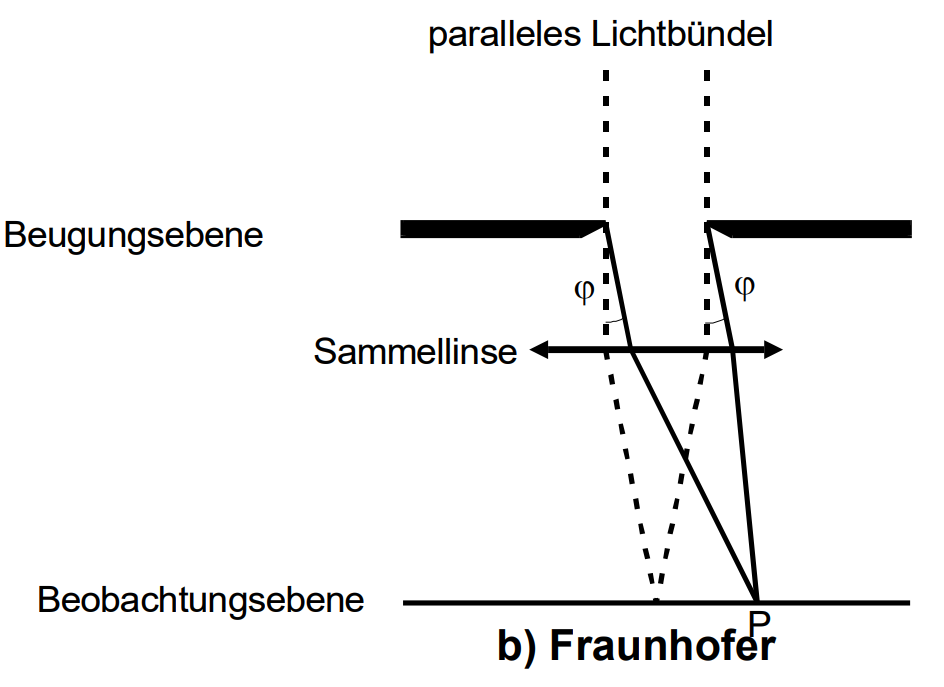
\includegraphics[width=260pt]{data/fraunhofer.png}
  \caption{Skizze der Fraunhofer-Beugung \cite{Versuchsanleitung}.}
  \label{fig:fraunhofer}
\end{figure}

Die dargestellte Sammellinse dient zur Fokussierung der Strahlen in einer Brennebene,
sodass der Winkel aller im Punkt P interferierenden Strahlen gleich wird.

%hier fange ich dann mal mit den Formeln aus der Anleitung an

Die Beugung am Spalt unter der Fraunhofer-Näherung kann mithilfe des Huygens'schen
Prinzips verstanden und veranschaulicht werden. Dieses erlaubt die Auffassung einer
Wellenfront als Einhüllende von unendlich vielen Elementarwellen. Von jedem Punkt
einer Wellenfront geht eine kugelförmige Elementarwelle aus, die sich mit gleicher Amplitude und
Frequenz ausbreitet, wie die ursprüngliche Welle. Die Einhüllende aller Elementarwellen
zu einem Zeitpunkt ergibt dann die neue Wellenfront.
Das Interferenzmuster auf dem Schirm ergibt sich durch aufgrund ihres Wegunterschiedes
entstehende Phasenunterschiede der Wellen. Durch gemoetrische Beziehungen in
Abbildung \ref{fig:gangunterschied} lässt sich für die Phasendifferenz die
Beziehung
\begin{equation}
  \delta = \frac{2\pi s}{\lambda} = \frac{2 \pi x \sin(\phi)}{\lambda} \,.
\end{equation}
Die Bedeutung der Bezeichnungen können der Abbildung entnommen werden.

\begin{figure}
  \centering
  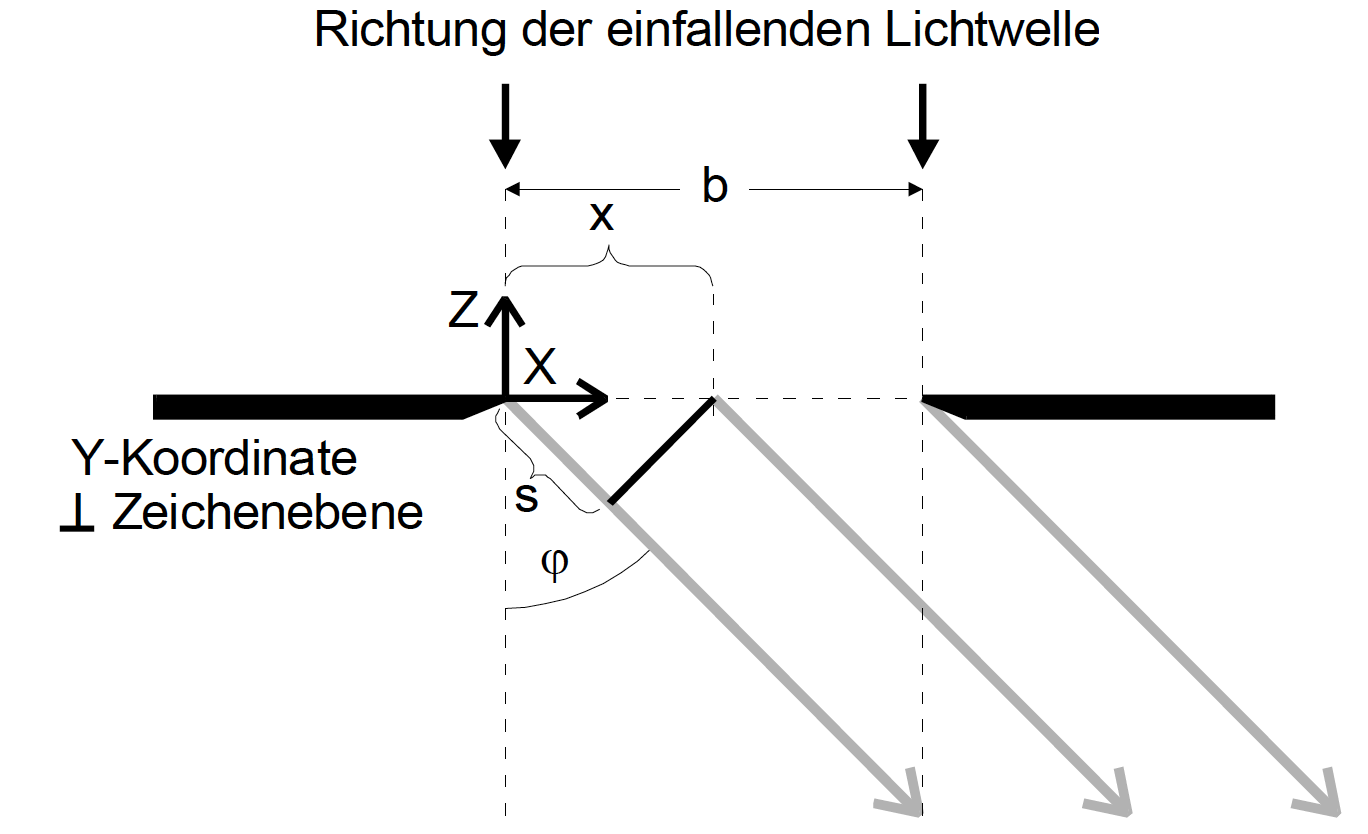
\includegraphics[width=260pt]{data/gangunterschied.png}
  \caption{Skizze für die Herleitung des Gangunterschiedes \cite{Versuchsanleitung}.}
  \label{fig:gangunterschied}
\end{figure}


Mithilfe dieser Beziehung lässt sich eine Beziehung für
die Feldstärke des Beugungsbildes des Einfachspaltes in Abhängigkeit vom Ablenkwinkel herleiten:
\begin{equation}
  B(\phi)= A_0 b \, \symup{sinc}\biggl(\frac{\pi b \sin(\phi)}{\lambda}\biggr) \,.
\end{equation}
Dabei ist $A_0$ die maximale Ampplitude der Funktion, $b$ die Breite des Spaltes,
und $\phi$ der Ablenkwinkel. Zudem gilt hier die Definition $\symup{sinc}(x)=\frac{\sin(x)}{x}$.
Da die Feldstärke im Versuch aufgrund der hohen Frequenz der Lichtwellen nicht gemessen
werden kann, wird die Intensität gemessen. Diese folgt dem Zusammenhang
\begin{equation}
  I_{\symup{einzel}}(\phi) \propto B_{\symup{einzel}}(\phi)^2=A_0^2 b^2 \symup{sinc}^2\biggl(\frac{\pi b \sin(\phi)}{\lambda}\biggr)  \,.
\end{equation}

Für die Intensität des Beugungsbildes eines Doppelspaltes ergibt sich
\begin{equation}
  I_{\symup{doppel}}(\phi) \propto 4 \cos^2\biggl(\frac{\pi s \sin(\phi)}{\lambda}\biggr)B_{\symup{einzel}}(\phi)^2 \,.
\end{equation}
Hierbei gelten die zuvor bereits erläuterten Bezeichnungen weiterhin. $s$ steht für
den Abstand der Spalte zueinander. Die Einhüllende dieser Verteilung ist das
Beugungsmuster des Einzelspaltes. Die Anzahl der Oszillationen darunter steigt mit
größerem Abstand und geringerer Größe der Spalte.

Da im gesamten Versuch die Fraunhofer-Näherung angenommen wird, gilt die Kleinwinkelnäherung,
sodass für den Ablenkwinkel die Gleichung
\begin{equation}
  \phi \approx \tan(\phi)=\frac{x-x_0}{L}
\end{equation}
gilt. Dabei ist $x$ die Position des Detektors, $x_0$ die Position des nullten Maximums
und $L$ der Abstand vom Spalt zum Detektor.

Es lässt sich zeigen, dass das Beugungsbild und die Gestalt des beugenden Objekts über eine
Fouriertransformation zusammenhängen.



%Bestimmt sind Teile noch brauchbar, also lasse ich es erstmal drin

%Es stellt sich heraus, dass die komplexe Amplitude $U$ an dem Beobachtungsort
%$\symbf{r}_p$ für Fraunhofersche Beugung an einer Öffnung der Fläche $A$
%ohne phasenverschiebendes Material durch
%\begin{equation}
%  U(\symbf{r}_p) = C' \int_{A} \symup{d}x \, \symup{d}y \, e^{-i(\symbf{q} \cdot \symbf{r})}
%  \label{eqn:beugungsintegral}
%\end{equation}
%gegeben ist. Dies ist die zweidimensionale asymmetrische Fouriertransformierte der
%Blende. Der Streuvektor $\symbf{q} = {\symbf{k}}_\text{aus} - {\symbf{k}}_\text{ein}$
%gibt die Differenz der Wellenzahlen der einfallenden und der ausfallenden Welle ein.
%Die Konstante $C'$ enthält Informationen über die Phase der Welle und dass die Beugung
%eine Kugelwelle hervorruft. Der Beobachtungsschirm befindet sich in der ($x$,$y$)-Ebene.
%Ausführung der Integration über einen Spalt der Breite $2a$ führt auf die Amplitude
%\begin{equation}
%  U(\symbf{r}_p) = 4 \pi C' a \delta(q_y) \frac{\sin(q_x a)}{q_x a}\,.
%\end{equation}
%Die Deltadistribution beschreibt, dass die Ausbreitung der Welle in y-Richtung durch den
%Spalt nicht beeinflusst wird. Die Amplitude der Welle ist nicht in einem Experiment nicht
%direkt messbar, da ihre Frequenz zu hoch ist. Stattdessen wird die Intensität gemessen.
%Diese ist proportional zum Quadrat der Amplitude. Wird der Ablenkwinkel $\beta$ mit
%\begin{equation*}
%  q_x a = k a \sin(\beta)
%\end{equation*}
%eingeführt, ergibt sich für die Intensität als Funktion des Ablenkwinkels
%\begin{equation}
%  I = I(\beta = 0) \frac{\sin^2(k a \sin \beta)}{(k a \sin \beta)^2}\,.
%\end{equation}
%Dabei ist $I(\beta = 0)$ die maximale Intensität der nicht abgelenkten Welle.
%Dazu analog erfolgt die Berechnung der Intensitätsverteilung an einem Doppelspalt.
%Wieder betrage die Breite eines Spaltes $2a$, der Abstand der Mittelpunkte sei
%$d > 2a$. Für die Intensitätsverteilung ergibt sich
%\begin{equation}
%  I = I(\beta = 0) \frac{\sin^2(k a \sin \beta)}{(k a \sin \beta )^2} 4 \cos^2 \left (\frac{k d}{2} \sin \beta \right)\,.
%\end{equation}
%Die Einhüllende dieser Verteilung ist das Beugungsmuster des Einzelspaltes. Die Anzahl
%der Oszillationen darunter steigt mit größerem Abstand und geringerer Größe der Spalte.
%Der Gedankengang der Herleitung und die Formeln entstammen \cite{Stolze}.
%
